\subsection{Eerste- en tweedegraadsfuncties}

\subsubsection{Constante functies}

\emph{Definitie}

Functievoorschrift: $f(x)=a$ met $a\in\mathbb{R}$

%\noindent \uline{Voorbeeld}: $f(x)=2$

Grafische voorstelling van de constante functie
met vergelijking $f(x)=a$ is een horizontale rechte, waarbij de $y$-as
wordt gesneden in het punt $(0,a)$.

%\noindent Alle afgeleiden zijn overal nul, er zijn geen extrema, geen
%buigpunten...

Tekenverloop: Zie Tabel \ref{tab:ct}.

\begin{table}[h]
	\centering\begin{tabular}{c||c}
		$x$ & \\
		\hline 
		$f(x)$ & teken van $a$\\
	\end{tabular}
	\caption{Tekenverloop van een constante functie.}
	\label{tab:ct}
\end{table}

\emph{Voorbeeld}

Gegeven de functie: $f(x)=\frac{1}{2}$, zie Figuur \ref{fig:ct}. 

Grafische voorstelling:
\begin{itemize}
\item het domein van de constante functie is altijd: $\textrm{dom}f=\mathbb{R}$
\item het beeld van deze constante functie is: $\textrm{bld}f=\frac{1}{2}$
\end{itemize}
\begin{figure}[h]
\centering{}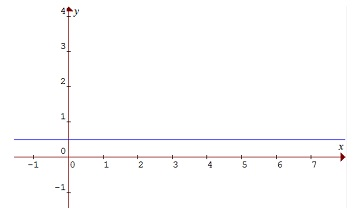
\includegraphics[height=5cm]{2_elem_rekenvaardigheden_B/inputs/constantefuncties.jpg} 
\caption{Voorbeeld constante functie.}
\label{fig:ct}
\end{figure}

Tekenverloop
Zie Tabel \ref{tab:ct_vb}.
\begin{table}[h]
\centering
\begin{tabular}{c||c}
	$x$ & \\
	\hline 
	$f(x)$ & $+$ \\
\end{tabular}
\caption{Voorbeeld tekenverloop constante functie.}
\label{tab:ct_vb}
\end{table}


\subsubsection{Eerstegraadsfuncties of lineaire functies}


\emph{Definitie}

Functievoorschrift: $f(x)=ax+b$ met $a\in\mathbb{R}_{0}$
en $b\in\mathbb{R}$.

\emph{Voorbeelden}

 $f(x)=10x+1$ , $f(x)=8-5x$ , $f(x)=3x$

\emph{Grafische voorstelling van de lineaire functie
	is een rechte.} 
Zie Figuur \ref{fig:eerstegr}.

\begin{figure}[h]
\centering{}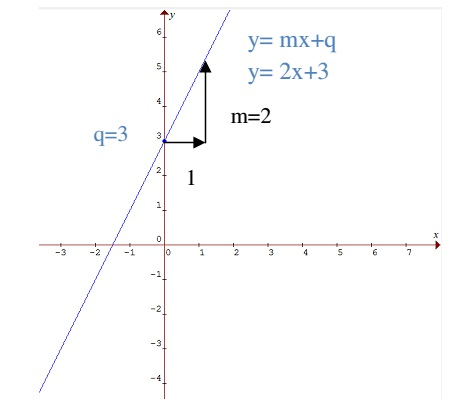
\includegraphics[height=5cm]{2_elem_rekenvaardigheden_B/inputs/eerstegraadsfuncties1.jpg} 
\caption{Voorbeeld van een eerstegraadsfunctie.}
\label{fig:eerstegr}
\end{figure}

\begin{itemize}
	\item Het domein van elke lineaire functie is: $\textrm{dom} f = \mathbb{R}$.
	\item Het beeld van deze lineaire functie is: $\textrm{bld} f = \mathbb{R}$.
\end{itemize}

\noindent De rechte wordt bepaald door de \textbf{richtingsco\"effici\"ent}
(de \textbf{rico}) \textquoteleft $a$\textquoteright{} en de intercept
\textquoteleft $b$\textquoteright . De rico bepaalt de helling van
de rechte. Als $x$ met 1 eenheid toeneemt, dan neemt $y$ met $a$
eenheden toe. Hoe groter de absolute waarde van de rico $a$, hoe
steiler de rechte.
\begin{itemize}
\item een positieve rico, hoort bij een stijgende rechte
\item een negatieve rico hoort bij een dalende rechte
\end{itemize}
\begin{figure}[h]
\centering{}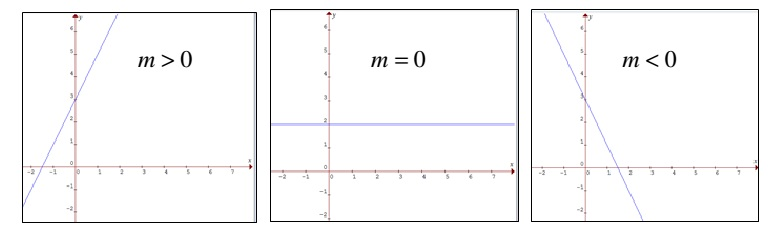
\includegraphics[width=\linewidth]{2_elem_rekenvaardigheden_B/inputs/eerstegraadsfuncties2.jpg} 
\caption{Het teken van de rico bepaalt of de rechte stijgt, constant is of daalt.}
\label{fig:rico}
\end{figure}

Zie Figuur \ref{fig:rico}.

\noindent Een rechte evenwijdig met de $x$-as heeft een rico gelijk
aan 0. Dit is in feite de constante functie $f(x)=b$.

\noindent Een rechte evenwijdig met de $y$-as heeft geen rico (in
dit geval zou $m=\infty$ moeten zijn). 

Nulpunten: het snijpunt met de $x$-as is het
punt $(-\frac{b}{a},0)$.

%\noindent \uline{De eerste afgeleide} van $f(x)$ is $f^{'}(x)=(mx+b)^{'}=m$.
%Dit betekent dat de eerste afgeleide ons meteen vertelt of het om
%een stijgende of een dalende rechte gaat.
%
%\noindent Er zijn geen extrema, geen buigpunten...

Tekenverloop: Zie Tabel \ref{tab:eerst_agr0} en \ref{tab:eerst_akl0}.
\begin{table}[h]
	\centering\begin{tabular}{c||c|c|c}
		$x$ &  & $-\frac{b}{a}$ & \\
		\hline 
		$f(x)$ & - & 0 & +\\
	\end{tabular}
\caption{Tekenverloop voor $a>0$.}
\label{tab:eerst_agr0}
\end{table}

\begin{table}[h]
	\centering\begin{tabular}{c||c|c|c}
		$x$ &  & $-\frac{b}{a}$ & \\
		\hline 
		$f(x)$ & + & 0 & -\\
	\end{tabular}
	\caption{Tekenverloop voor $a<0$.}
	\label{tab:eerst_akl0}
\end{table}

\emph{Voorbeeld}

Gegeven de functie: $f(x)=-2x+3$, zie Figuur \ref{fig:eerste_vb_graf}.

Grafische voorstelling:
\begin{itemize}
\item het domein van elke lineaire functie is: $\textrm{dom}f=\mathbb{R}$
\item het beeld van deze lineaire functie is: $\textrm{bld}f=\mathbb{R}$
\end{itemize}
\begin{figure}[h]
\centering{}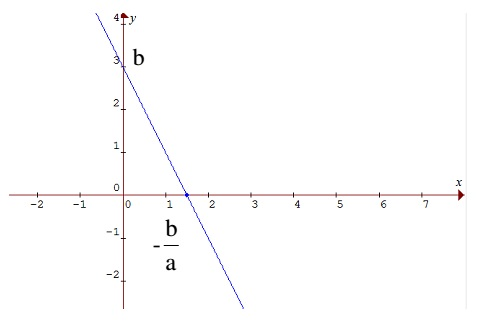
\includegraphics[height=5cm]{2_elem_rekenvaardigheden_B/inputs/eerstegraadsfuncties3.jpg}
\caption{Voorbeeld grafische voorstelling van de eerstegraadfunctie.}
\label{fig:eerste_vb_graf} 
\end{figure}


Nulpunten:

\noindent We lossen de vergelijking $y=f(x)=-2x+3=0$ op en vinden:
$x=\frac{3}{2}$. Het snijpunt met de $x$-as is het punt $(\frac{3}{2},0)$.

Tekenverloop: zie Tabel \ref{tab:eerste_vb}.

\begin{table}[h]
\centering
\begin{tabular}{c||c|c|c}
	$x$ &  & $\frac{3}{2}$ & \\
	\hline 
	$f(x)$ & $+$ & 0 & $-$\\
\end{tabular}
\caption{Voorbeeld eerstegraadsfunctie: tekenverloop}
\label{tab:eerste_vb}	
\end{table}


\subsubsection{Tweedegraadsfuncties of kwadratische functies}


\emph{Definitie}

Functievoorschrift: $f(x)=ax^{2}+bx+c$ met $a\in\mathbb{R}_{0}$
en $b,c\in\mathbb{R}$ 

\emph{Voorbeelden}
$f(x)=3x^{2}+10x+1$ , $f(x)=-2x^{2}+5$
, $f(x)=x^{2}$

\emph{Grafische voorstelling van de kwadratische functie
is een parabool.}
Zie Figuur \ref{fig:tweede}
\begin{figure}[h]
\centering{}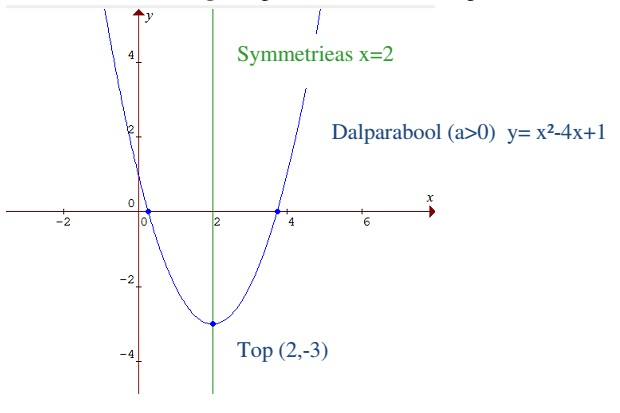
\includegraphics[width=.7\linewidth]{2_elem_rekenvaardigheden_B/inputs/tweedegraadsfuncties1.jpg}
\caption{Grafische voorstelling van een tweedegraadsfunctie.}
\label{fig:tweede} 
\end{figure}

\begin{itemize}
\item \noindent als $a>0$ is de top van de \textbf{dalparabool} het minimum
\item \noindent als $a<0$ is de top van de \textbf{bergparabool} het maximum
\end{itemize}
\noindent Hoe groter de absolute waarde van $a$, hoe smaller de opening
van de parabool is.

De verticale lijn door de top is de \textbf{symmetrieas}.
De vergelijking van de symmetrieas is: $x=-\frac{b}{2a}$ 

Het laagste punt van een dalparabool of het hoogste punt
van een bergparabool heet de \textbf{top} van de parabool. De top
is het snijpunt van de parabool met de verticale symmetrieas. De co\"ordinaten
van de top zijn dus $(-\frac{b}{2a},y)$. De $y$-waarde vinden we
door de gevonden $x$-waarde in het functievoorschrift $f(x)$ in
te vullen, dus $y=f(-\frac{b}{2a})$ .

Nulpunten: stellen we $y=f(x)=ax^{2}+bx+c=0$
(in dat geval spreken we van de \textbf{vierkantsvergelijking}), dan
vinden we de snijpunten met de $x$-as. Hiervoor moeten we dus de
(vierkants)vergelijking $ax^{2}+bx+c=0$ oplossen. Daarvoor bepaal
je best eerst de \textbf{discriminant} $D=b^{2}-4ac$ (van de abc
formule). Met de discriminant bepaal je het aantal snijpunten van
de kwadratische functie met de $x$-as, zie ook Figuur \ref{fig:tweede:gevallen}.
\begin{itemize}
\item als $D>0$ , dan heeft de vergelijking twee oplossing: $x_{1}=\frac{-b+\sqrt{D}}{2a}$
en $x_{2}=\frac{-b-\sqrt{D}}{2a}$. De parabool snijdt de $x$-as
op twee plaatsen.
\item als $D=0$ , dan heeft de vergelijking \'e\'en oplossing: $x_{1}=x_{2}=-\frac{b}{2a}$.
De parabool raakt met zijn top de $x$-as in \'e\'en punt.
\item als $D<0$ , dan heeft de vergelijking geen re\"ele oplossingen. De
parabool ligt ofwel boven ofwel onder de $x$-as.
\end{itemize}
\begin{figure}[h]
\centering{}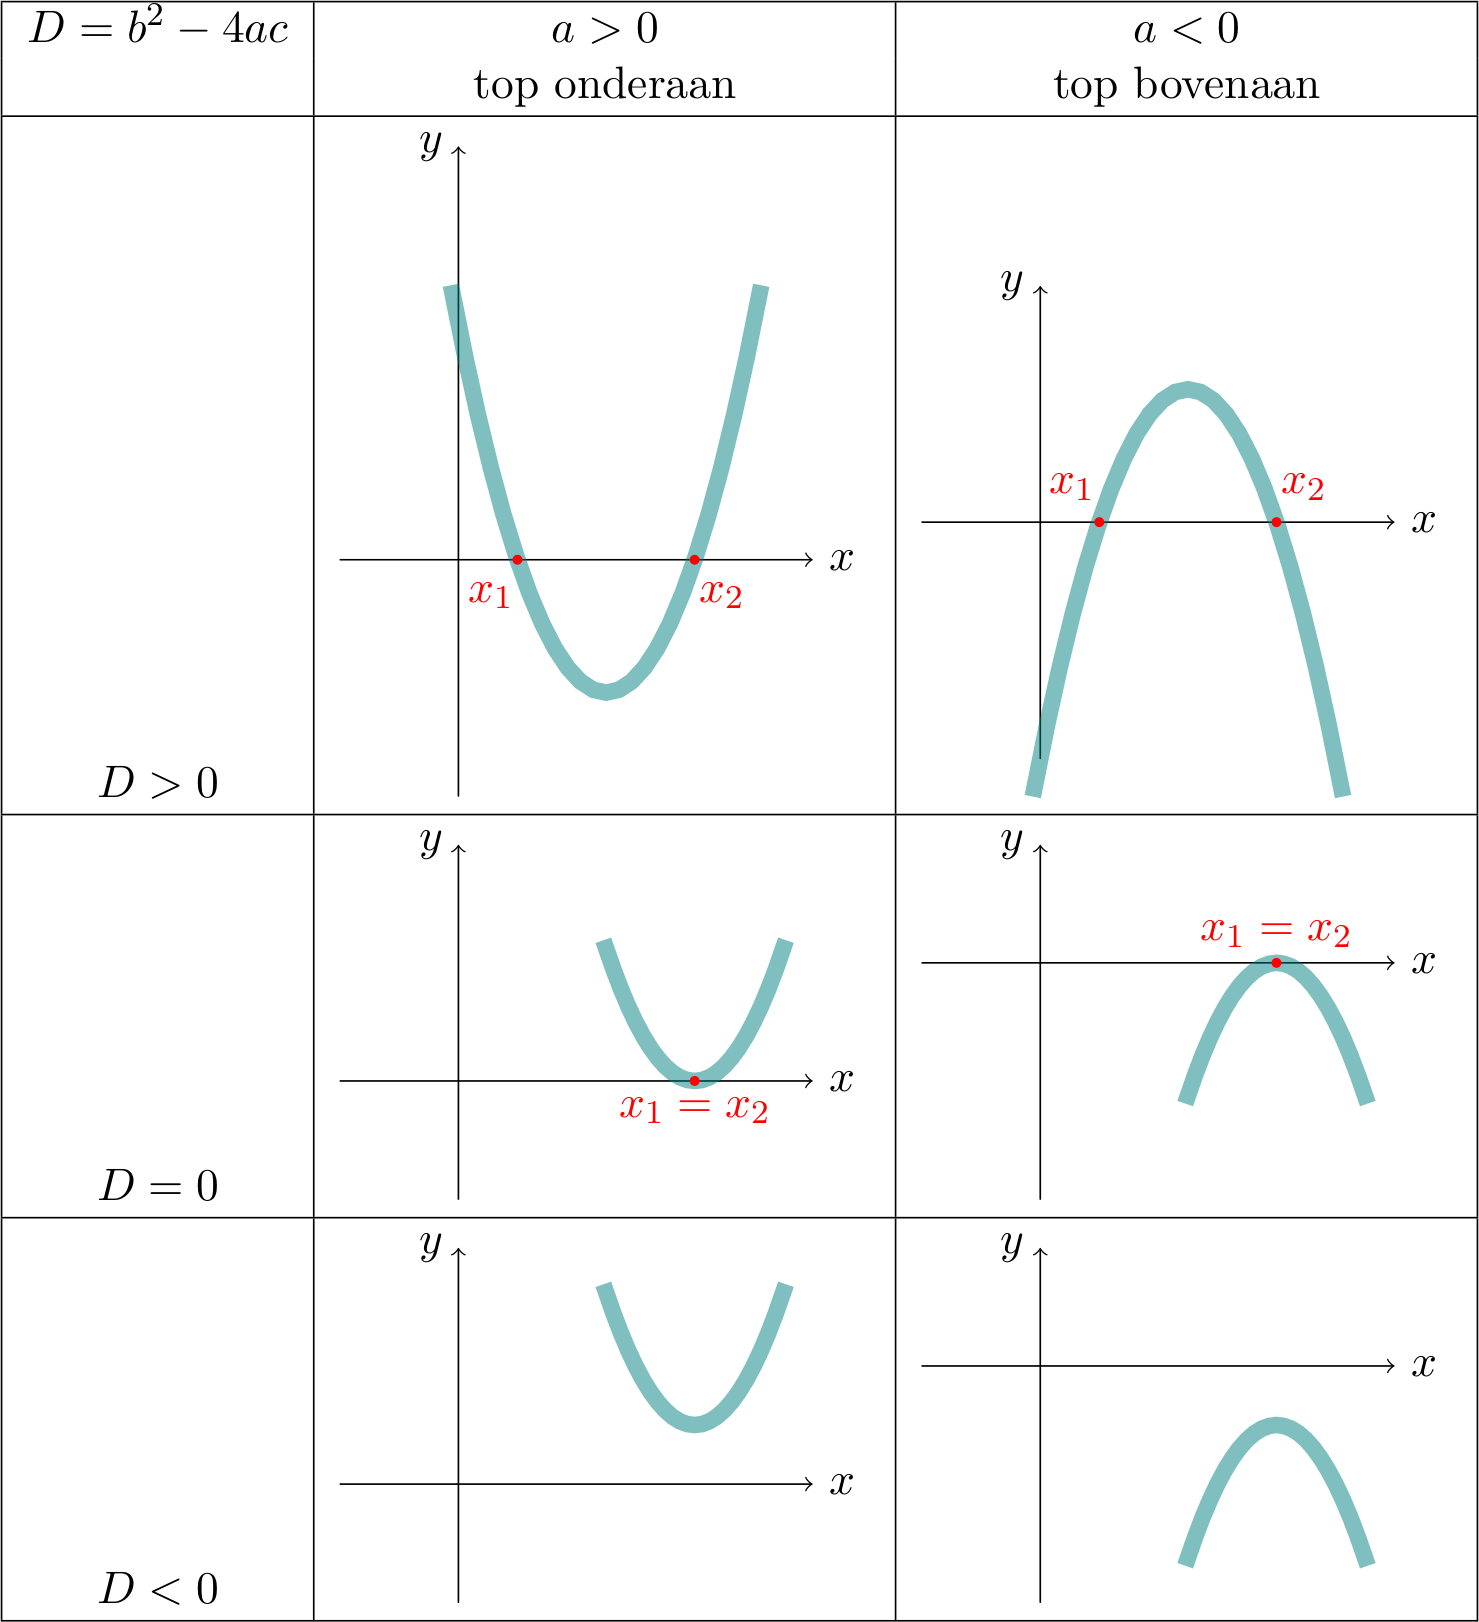
\includegraphics[scale=0.5]{2_elem_rekenvaardigheden_B/inputs/tweedegraadsfuncties2.jpg} 
\caption{Grafische voorstelling van tweedegraadsfuncties voor verschillende waarden van $a$ en $D$.}
\label{fig:tweede:gevallen}
\end{figure}


%\noindent \uline{Opmerking}: stellen we de eerste afgeleide gelijk
%aan nul, dan vinden we de $x$-co\"ordinaat van de top: $f^{'}(x)=(ax^{2}+bx+c)^{'}=2ax+b=0$
%of $x=-\frac{b}{2a}$ . Het teken van de eerste afgeleide zegt ons
%of de functie (links en rechts van de top) stijgt of daalt. Tenslotte,
%het teken van de tweede afgeleide $f^{''}(x)=(2ax+b)^{'}=2a$, m.a.w.
%het teken van $a$ , zegt ons of het om een dal- of bergparabool gaat.

Tekenverloop:

\begin{itemize}
\item Als $D>0$ \\
\begin{tabular}{c||c|c|c|c|c}
$x$ &  & $x_{1}$ &  & $x_{2}$ & \\
\hline 
$f(x)$ & teken van $a$ & 0 & tegengesteld teken van $a$ & 0 & teken van $a$\\
\end{tabular}
\item Als $D=0$ \\
\begin{tabular}{c||c|c|c}
	$x$ &  & $x_{1}=x_{2}$ & \\
	\hline 
	$f(x)$ & teken van $a$ & 0 & teken van $a$\\
\end{tabular}
\item Als $D<0$ \\
\begin{tabular}{c||c}
$x$ & \\
\hline 
$f(x)$ & teken van $a$\\
\end{tabular}
\end{itemize}
%\begin{table}[h]
%\centering
%\caption{Algemeen tekenverloop van een tweedegraadsfunctie voor $D>0$}
%\end{table}
%\begin{tabular}{c|c}
%$D=0$ & %
%\begin{tabular}{c||c|c|c}
%$x$ &  & $x_{1}=x_{2}$ & \\
%\hline 
%\hline 
%$f(x)$ & teken van $a$ & 0 & teken van $a$\\
%\end{tabular}\\
% & \\
%\hline 
% & \\
%$D>0$ & %
%\begin{tabular}{c||c|c|c|c|c}
%$x$ &  & $x_{1}$ &  & $x_{2}$ & \\
%\hline 
%\hline 
%$f(x)$ & teken van $a$ & 0 & tegengesteld teken van $a$ & 0 & teken van $a$\\
%\end{tabular}\\
% & \\
%\hline 
% & \\
%$D<0$ & %
%\begin{tabular}{c||c}
%$x$ & \\
%\hline 
%\hline 
%$f(x)$ & teken van $a$\\
%\end{tabular}\\
%\end{tabular}


\emph{Voorbeeld}

Gegeven de functie $f$ met voorschrift: $f(x)=-x^{2}-5x+6$ 

Grafische voorstelling:
\begin{itemize}
\item het domein van elke kwadratische functie is: $\textrm{dom}f=\mathbb{R}$
\item $a=-1<0$ dus het is een bergparabool
\item de symmetrieas ligt bij $x=-\frac{b}{2a}=-\frac{-5}{2.(-1)}=-\frac{5}{2}=-2,5$
\item de top heeft de co\"ordinaten $(x,y)=(-\frac{b}{2a},f(-\frac{b}{2a}))=(-2,5;12,25)$
\item de top van deze bergparabool ligt op $y=12,25$. Dit is dus de grootste
waarde die $y$ kan bereiken. Het beeld van deze kwadratische functie
is daarom: $\textrm{bld}f=]-\infty;12,25]$
\end{itemize}


Nulpunten:

\noindent We lossen de vergelijking $y=f(x)=-x^{2}-5x+6=0$ op d.m.v.
de abc formule. We berekenen daarvoor eerst de discriminant $D$:

$D=b^{2}-4ac=(-5)^{2}-4.(-1).6=25+24=49$

\noindent Omdat $D>0$ zijn er 2 re\"ele oplossingen, dus 2 snijpunten
met de $x$-as. Deze zijn:
\begin{itemize}
\item $x_{1}=\frac{-b+\sqrt{D}}{2a}=\frac{-(-5)+\sqrt{49}}{2.(-1)}=-6$
\item $x_{2}=\frac{-b-\sqrt{D}}{2a}=\frac{-(-5)-\sqrt{49}}{2.(-1)}=1$
\end{itemize}
De parabool snijdt de horizontale as in de koppels (-6,0) en (1,0)
en de top ligt boven de $x$-as (want het is een bergparabool), zie ook Figuur \ref{fig:tweede:vb}.

\begin{figure}[h]
\centering{}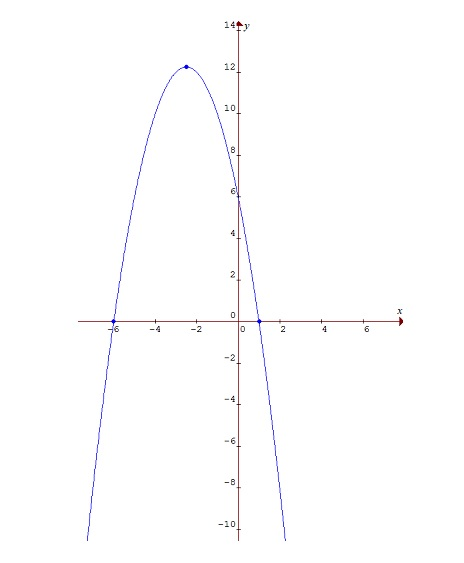
\includegraphics[width=.5\linewidth]{2_elem_rekenvaardigheden_B/inputs/tweedegraadsfuncties3.jpg}
\caption{Voorbeeld tweedegraadsfuncties: grafische voorstelling}
\label{fig:tweede:vb} 
\end{figure}


Tekenverloop:
Zie Tabel \ref{tab:tweede:vb}

\begin{table}[h]
	\centering
\begin{tabular}{c||c|c|c|c|c}
	$x$ &  & $-6$ &  & $1$ & \\
	\hline 
	$f(x)$ & $-$ & 0 & $+$ & 0 & $-$\\
\end{tabular}
\caption{Voorbeeld tweedegraadsfuncties: tekenverloop}
\label{tab:tweede:vb}	
\end{table}
